\chapter{System Description}
\label{chap:system_description}

In this chapter, the equipment used will be discussed in detail, including its integration and how it was modeled and implemented in both hardware and software. 
The python automation routine that is the focus of this project was started by a previous student\cite{Monica}, and the software itself was originally created as an electrospray multipurpose library.

\section{Hardware model}
\label{sec:hardware_model}

\subsection{Instrumentation}
\label{subsec:instrumentation}

The main instruments used for this project are listed below:

\begin{enumerate}[a)]

  \item High Voltage Power Supply (HVPS)
  
     - brand: FUG
    
     - model: HCP35-20kV
    
    The HVPS provides the electrical potential to the liquid, which can be applied by connecting the HVPS directly to the liquid feeding capillary or needle to a grounded electrode (usually a plate or a ring) located downstream.\cite{Monica}
    The setup has the USB serial interface for controlling and polling measurements.
    
    The software has an interface to integrate the HVPS to the routine. This interface can be found in \emph{FUG\_function.py} file where is located the functions used to control and collect data from this instrument.
    In case of change of equipment, a new interface must be created within this file to match another manufacturer specifications.

  \item Wireless Oscilloscope
  
     - Brand: \emph{TiePie engineering}

     - model: TiePie WifiScope WS6 DIFF
    
    The signal analysis with an oscilloscope using Wi-Fi technology allows an in-depth case study of the electric current signal.
    The current is measured via a TiePie WifiScope WS6 from TiePie engineering that is a battery powered oscilloscope capable of transmitting data via a Wi-Fi connection allowing it to be placed in the high voltage or ground path.
    
    Wireless communication allows measurements disconnected from an external power supply, which increases safety when using high voltage potential references and also reduce the signal noise collected from external power lines.
    The current is routed directly via the input, hence the oscilloscope measures the voltage dropped via its input resistance (which can be switched between 1 or 2 Mohms).
    TiePie WifiScope WS6 has a resolution of up to 16 bit at a minimal input range of 200 mV, sufficient to measure currents down to 1 nA. In addition the WifiScope has an open source interface library for python, \cite{TiePieLib}, making it easier to integrate with the automation routine.

  \item Humidity and Temperature sensor
  
  The stability of the system is affected by many physical effects. Evidently, it favors the system control having more parameters analyzed.
  The surface tension force, for example, is dependent of the liquid-gas interface on the meniscus, hence, the surrounding gas must be constant and so its humidity.
  Also, temperature is a variable that interferes in many phenomena in the system, specially the liquid properties such as viscosity.

  For that, a standard microcontroller development board (\emph{Arduino Uno}) with a temperature and humidity sensor (DHT11) was configured to add that data in real time to the routine.

  \item High Speed Camera 
  
  - Brand: \emph{Photron}

  - model: Photron fastcam mini

  The High Speed Camera (HSC) was just used in this project for validation purposes.
  
  \item Syringe pump
  
  - Brand: \emph{Master dual}

  - model: WPI AL-1000

  The pump integration in the automation algorithm was done in this work, bringing a new controllable variable, the flow rate. The spraying mode can be controlled using the two main variables that affect the system. 
  It brings more complexity for the system since now it is a multivariable control.
  Controlling also the flow rate provides this project a new dimension in the system giving freedom to explore the flow rate properties.
  With this new input variable the control system is MISO (Multiple Inputs Single Output).

  About the pump interface, as there was no good ready-to-use library, a simple and intuitive interface was developed to be used in the software routine.
  The communication protocol used is RS-232 and the pump commands list were found in the user manual.


  \end{enumerate}


Figure \ref{fig:setup} illustrates a diagram with all the key components in the system. The peripherals are connected to a computer running the software routine via serial communication. 
This diagram encapsulates the process system and will be used as a sub-system of the control model. The inputs in the process are power supply voltage and pump machine flow rate, referred here as the controller values. The output is the oscilloscope current measurement.

\begin{figure}[H]
  \centering
  \resizebox{150mm}{!}{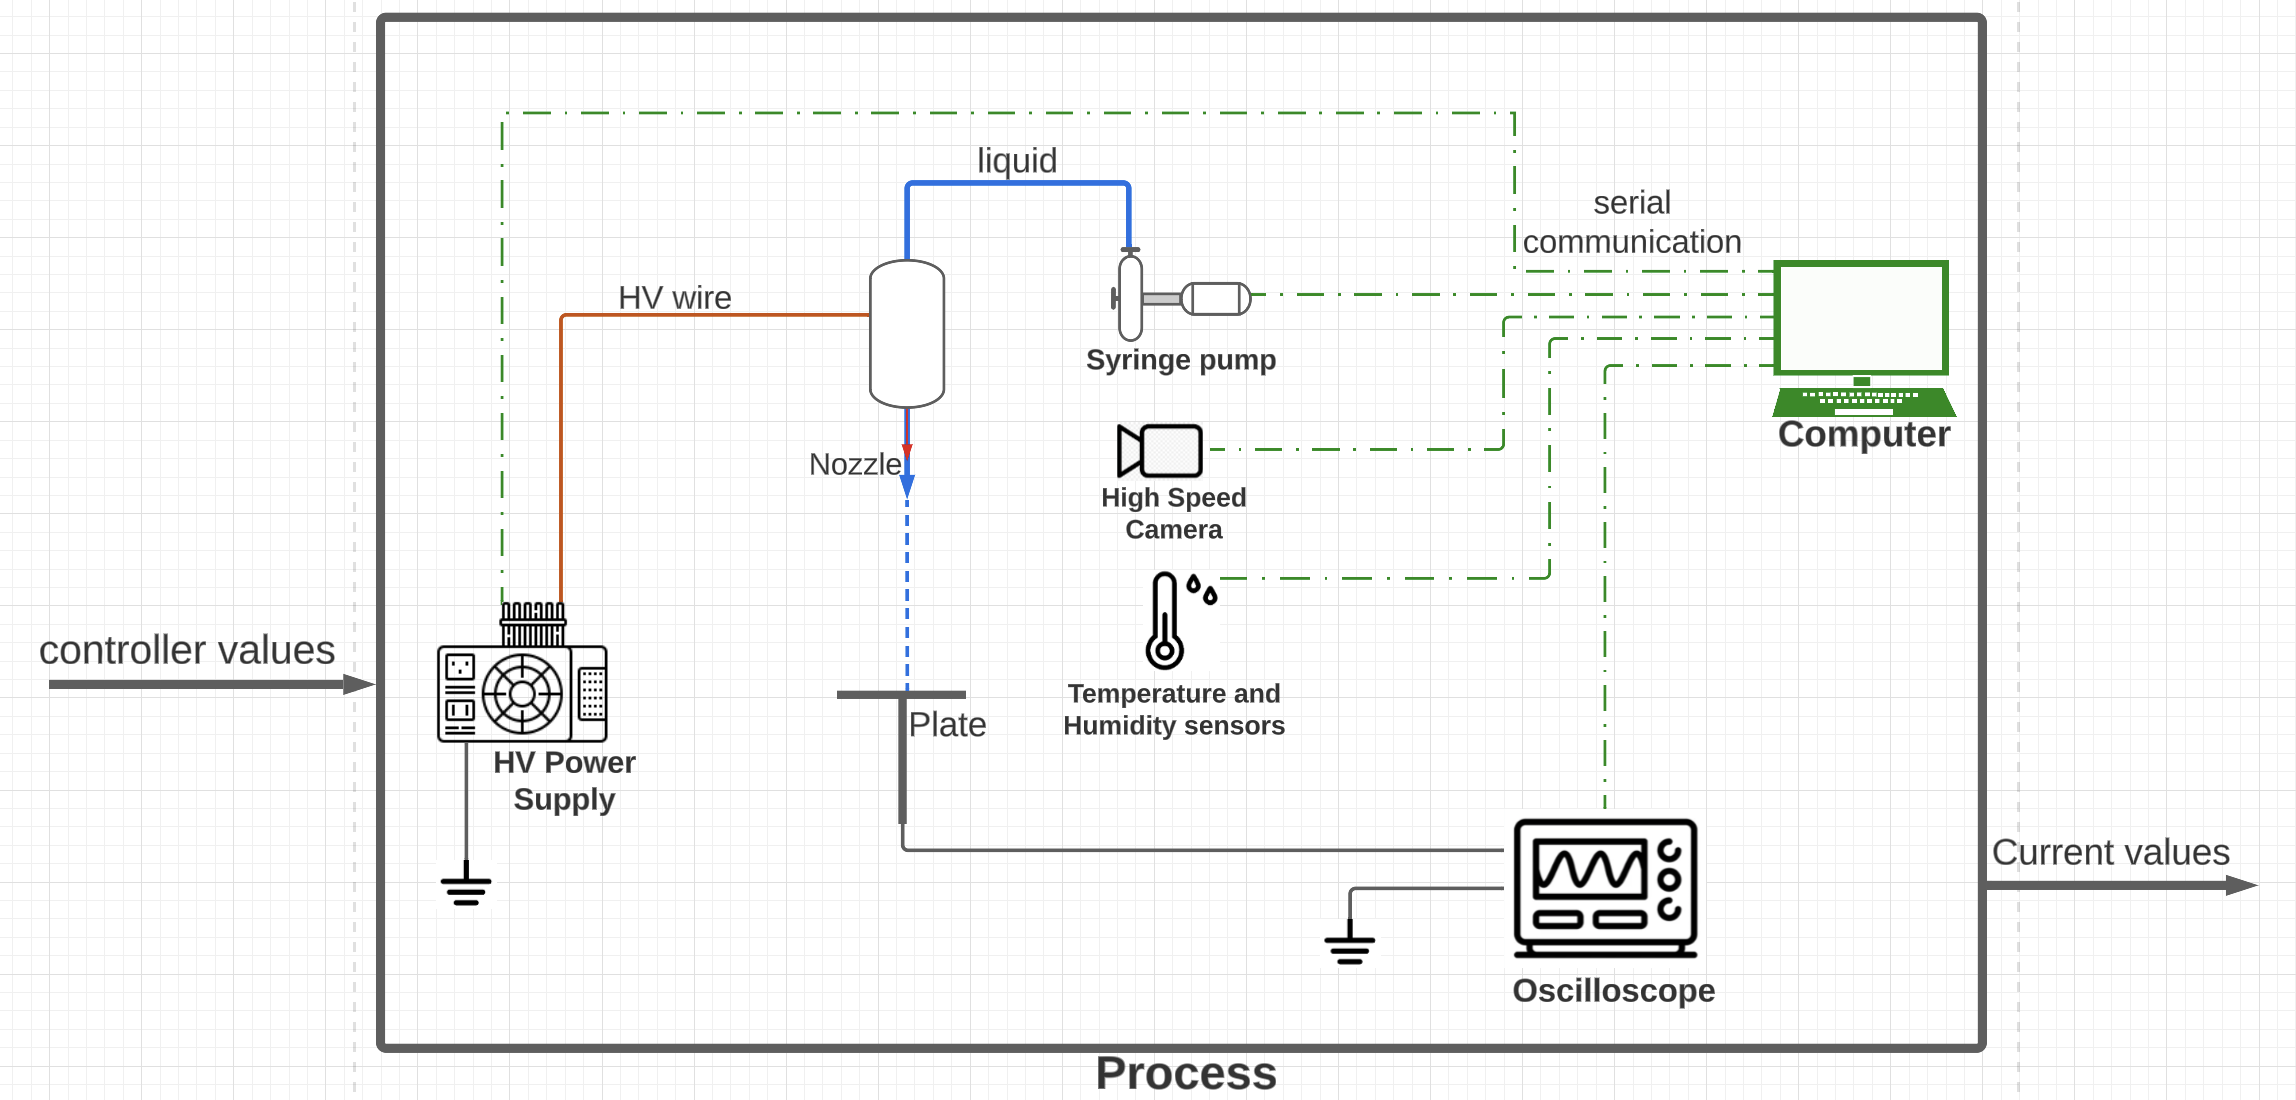
\includegraphics{Figuras/new_system_setup.png}}
  \caption{EHDA automation system setup.}
  \label{fig:setup}
\end{figure}

There are also many minor variables that affect the experiment stability. More details are explained in appendix \ref{sec:setup_validation}.


\section{Software Model}
\label{sec:control_model}

The software was reformulated on top of the control model represented in Figure \ref{fig:control_model_fig}. The process of the control loop is the same as represented in Figure \ref{fig:setup}. 
Each other subsystem in the control loop is a separate thread that will be explained below.

\begin{figure}[H]
  \centering
  \resizebox{150mm}{!}{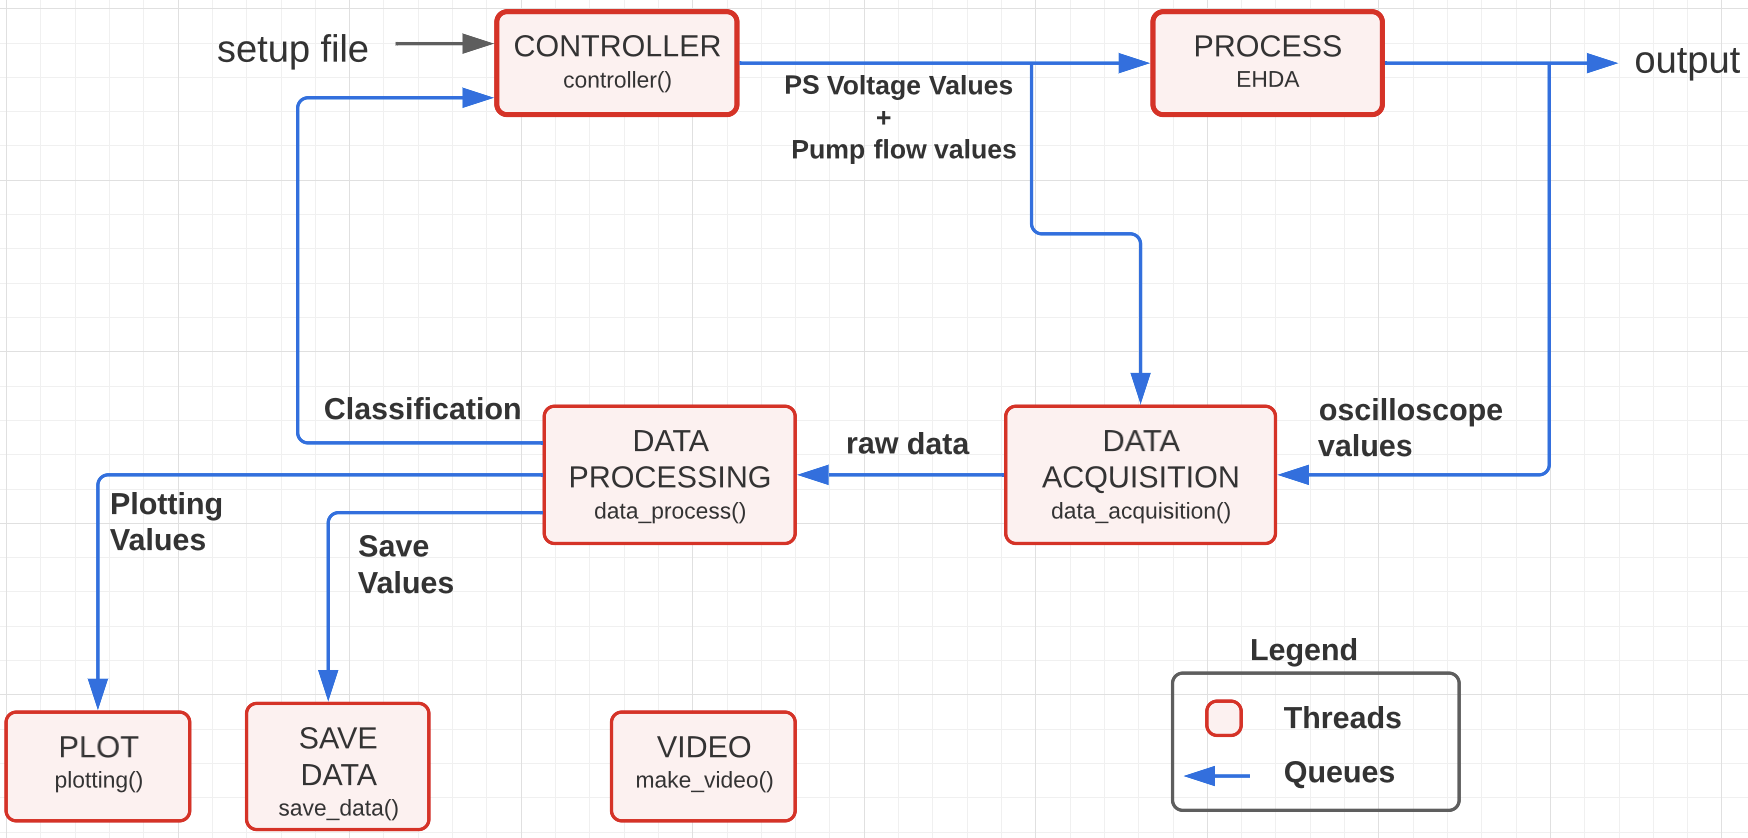
\includegraphics{Figuras/control_loop.png}}
  \caption{EHDA automation closed loop control system model implemented.}
  \label{fig:control_model_fig}
\end{figure}

\subsection{Threading and Queues}
\label{subsec:concurrency}

    In order to implement this closed loop control model in the software and explore parallel processing, each sub-system was implemented as a separate thread.
    For concurrency on flux of data between threads was used queues structures.
    A queue is an abstract data type that holds an ordered, linear sequence of items. You can describe it as a first in, first out (FIFO) structure.

    The controller thread is responsible for sending to the power supply the set voltage values and to syringe pump the flow rate set values according to the sequence selected.
    Also, responsible for sending the finish event command that end the routine and trigger the threads to close their routines.
    As input, the setup config file with information about the liquid and the setup used such as geometric parameters of the nozzle to plate system. As output, the commands to the actuators.

    The data acquisition thread is responsible for concatenating the current, voltage, flow rate, humidity and temperature data and concatenate it into one sample.
    The data processing is responsible for calculating the statistical values from the raw data and classify it in the respective spray mode for that sample.
    After processing, the data is saved in real time in a json file using \emph{jsonstreams} library to save one sample structure at a time.
    With the new streaming model of saving, instead of having all data together in program memory to be saved in the end, it is saving each sample in real time during the experiment.
    The data acquired in each sample of 0.5s is shown in Figure \ref{fig:data_sample}.

    \begin{figure}[H]
        \center
        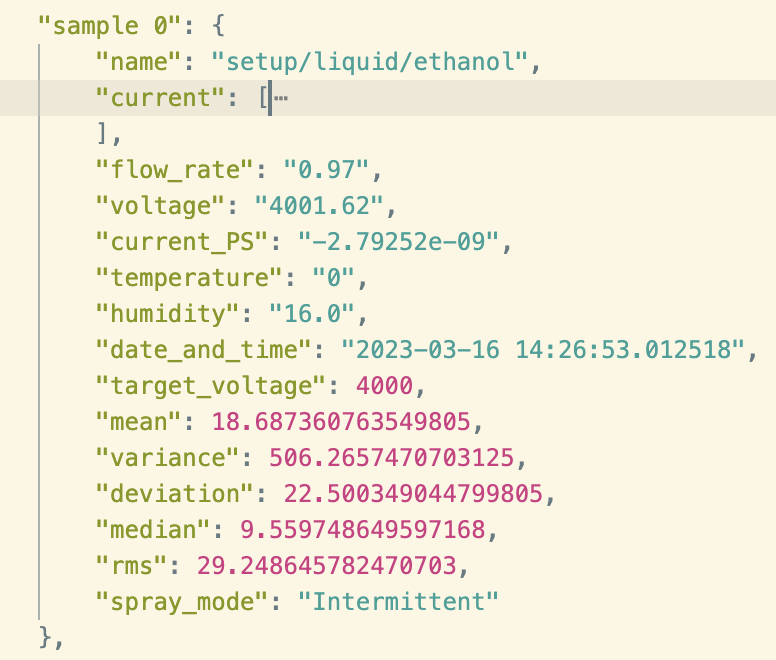
\includegraphics[width=10cm]{Figuras/19:03/new_sample.png}
        \caption{Output data json structure.}
        \label{fig:data_sample}
    \end{figure}

    This new way of saving the measurement and processing ensures that the data is stored separately in enumerated samples.
    This prevents any loss of data in the event of errors during experiments and significantly enhances the usability of the data for in-depth analysis. Each hour-long experiment generates approximately 6 GB of data, and effectively organizing such a substantial amount of data was a crucial enhancement in the software. To efficiently work with and analyze the data, the widely-used Python framework, pandas Dataframe, can be utilized with the following command:
    
    pandas.read\_json('PATH', orient='index').

    It will construct a Data frame with all data organized by samples.

    To conclude, json files are good as a system output because of its human readability. But as the database gets bigger json becomes slow to read and large to store. For that, saving the data frame in a compressed type of file called feather is much faster to work with it.

    This is only running function that should run in the main thread because of the plotting library \emph{matplotlib} incompatibilities with running outside the main function. 
    The plotting function is responsible for plotting in real time the current sample acquired, and its respective fast Fourier transform to evaluate the sample frequency spectrum.
    It takes as input the \emph{plot\_data\_queue} from the \emph{processing\_thread()} and displays three graphs updated in real time on the screen during the experiment.

  \section{Chapter conclusion}

    In this chapter it is explained the system description, detailing the hardware instruments, how it was modelled and its implementation in the software. 


\clearpage